\documentclass[aspectratio=169]{beamer}

% ── Base theme ──────────────────────────────────────────────────────────────
\usetheme{Madrid}
\setbeamertemplate{navigation symbols}{}

% ── Brand colors ─────────────────────────────────────────────────────────────
\definecolor{fptOrange}{HTML}{F37021}
\definecolor{fptNavy}{HTML}{1A2B4A}
\definecolor{fptLight}{HTML}{FFF5EE}
\definecolor{positive}{HTML}{0173B2}
\definecolor{negative}{HTML}{DE8F05}
\definecolor{emphasis}{HTML}{029E73}
\definecolor{neutral}{gray}{0.55}
\definecolor{cbPurple}{HTML}{CC78BC}

% ── Color palette ────────────────────────────────────────────────────────────
\setbeamercolor{palette primary}{bg=fptNavy,fg=white}
\setbeamercolor{palette secondary}{bg=fptNavy!80,fg=white}
\setbeamercolor{palette tertiary}{bg=fptOrange,fg=white}
\setbeamercolor{palette quaternary}{bg=fptNavy,fg=white}
\setbeamercolor{structure}{fg=fptOrange}
\setbeamercolor{frametitle}{bg=fptNavy,fg=white}
\setbeamercolor{title}{bg=fptNavy,fg=white}
\setbeamercolor{subtitle}{fg=fptOrange}
\setbeamercolor{section in toc}{fg=fptNavy}
\setbeamercolor{normal text}{fg=fptNavy}
\setbeamercolor{block title}{bg=fptNavy!10,fg=fptNavy}
\setbeamercolor{block body}{bg=fptNavy!4,fg=fptNavy}
\setbeamercolor{block title alerted}{bg=fptOrange!20,fg=fptOrange!80!black}
\setbeamercolor{block body alerted}{bg=fptOrange!6,fg=fptNavy}
\setbeamercolor{block title example}{bg=emphasis!15,fg=emphasis!70!black}
\setbeamercolor{block body example}{bg=emphasis!4,fg=fptNavy}

% ── Fonts ────────────────────────────────────────────────────────────────────
\usepackage{fontspec}
\setbeamerfont{title}{size=\Large,series=\bfseries}
\setbeamerfont{subtitle}{size=\normalsize,series=\normalfont}
\setbeamerfont{frametitle}{size=\large,series=\bfseries}
\setbeamerfont{block title}{size=\normalsize,series=\bfseries}

% ── Packages ─────────────────────────────────────────────────────────────────
\usepackage{amsmath,amssymb,booktabs,array}
\usepackage{graphicx}
\usepackage{tikz}
\usetikzlibrary{arrows.meta,positioning,shapes.geometric}
\usepackage{eso-pic}

% ── Kill Madrid's section headline bars ──────────────────────────────────────
\setbeamertemplate{headline}{}

% ── Frametitle with logo (full-width hbox, guaranteed visible) ────────────────
\setbeamertemplate{frametitle}{%
  \nointerlineskip%
  \begin{beamercolorbox}[wd=\paperwidth,ht=1.1cm,dp=0.2cm,leftskip=8pt,rightskip=8pt]{frametitle}%
    \usebeamerfont{frametitle}\color{white}\insertframetitle%
    \hfill%
    
\includegraphics[height=0.88cm]{../../docs/logo/fpt_logo.png}%
  \end{beamercolorbox}%
  \begin{beamercolorbox}[wd=\paperwidth,ht=2pt,dp=0pt]{palette tertiary}%
  \end{beamercolorbox}%
}

% ── Custom footline ───────────────────────────────────────────────────────────
\setbeamertemplate{footline}{%
  \leavevmode%
  \begin{beamercolorbox}[wd=\paperwidth,ht=2.5ex,dp=1.2ex,leftskip=8pt,rightskip=8pt]{palette primary}%
    \usebeamerfont{footline}\footnotesize
    \insertshortauthor\hfill
    \insertshorttitle\hfill
    \insertframenumber\,/\,\inserttotalframenumber\hspace{4pt}
  \end{beamercolorbox}%
}

\newcommand{\pos}[1]{\textcolor{positive}{#1}}
\newcommand{\con}[1]{\textcolor{negative}{#1}}
\newcommand{\HL}[1]{\textcolor{emphasis}{#1}}

\newcommand{\backupbegin}{%
  \newcounter{framenumberappendix}%
  \setcounter{framenumberappendix}{\value{framenumber}}%
}
\newcommand{\backupend}{%
  \addtocounter{framenumberappendix}{-\value{framenumber}}%
  \addtocounter{framenumber}{\value{framenumberappendix}}%
}

\title[Vietnamese GraphRAG --- Multi-hop QA]{Vietnamese GraphRAG\\Multi-hop Question Answering over Wikipedia}
\subtitle{Capstone Review 1 --- FPT University SE+AI}
\author[Trung, Anh, Khoi, Thien]{%
  Huynh Quoc Trung (QE180038) \and
  Nhu Quang Anh (QE180005) \and
  Pham Ngo Dinh Khoi (QE180110) \and
  Truong Dinh Thien (QE180018)
}
\institute{FPT University\\[4pt]\small\textit{Supervisors:} Lê Trung Hiếu \quad Đặng Nguyên Bình}
\date{Week 6 --- June 2026}

\begin{document}

% SLIDE 1: Title
\begin{frame}[plain]
\titlepage
\end{frame}

% SLIDE 2: Table of Contents
\begin{frame}{Table of Contents}
\begin{columns}[T]
\column{0.48\textwidth}
\begin{enumerate}
  \item Problem \& Objectives
  \item Users \& Practical Applicability
  \item Innovation \& New Technology
  \item System Architecture
  \item Requirements \& SRS
  \item AI: Problem Framing
\end{enumerate}
\column{0.48\textwidth}
\begin{enumerate}
  \setcounter{enumi}{6}
  \item Dataset
  \item Related Works (3 papers)
  \item AI Pipeline
  \item Evaluation Metrics
  \item Team Assignment
  \item System Scale \& Timeline
\end{enumerate}
\end{columns}
\end{frame}

% SLIDE 3: Problem Statement
\begin{frame}[shrink=12]{1. Problem Statement}
\begin{alertblock}{Core Challenge}
{\small\textbf{Complex questions} about Vietnamese history, geography, and people often \textbf{span multiple Wikipedia articles} --- impossible to answer with a single search.}
\end{alertblock}
\vspace{0.15em}
\begin{center}
\small
\begin{tabular}{l>{\raggedright\arraybackslash}p{6.8cm}}
\toprule
\textbf{User} & \textbf{Problem} \\
\midrule
Students / researchers & Must read 5--10 articles to synthesize an answer \\
Standard RAG systems & Only retrieves the nearest chunk --- loses multi-hop links \\
Vanilla LLMs & Hallucinate Vietnamese facts, no verifiable citations \\
\bottomrule
\end{tabular}
\end{center}
\vspace{0.15em}
\begin{exampleblock}{Research Gap}
{\small No publicly available Vietnamese GraphRAG system supports \textbf{multi-hop reasoning} over Wikipedia with \textbf{explainable citations}.}
\end{exampleblock}
\vspace{0.1em}
\begin{block}{Project Goal}
{\small\textbf{Build a fully local Vietnamese KGQA system} that answers multi-hop questions with validated citations, with no dependency on external APIs.}
\end{block}
\end{frame}

% SLIDE 4: Users & Practical Applicability
\begin{frame}[shrink=5]{2. Users \& Practical Applicability}
\begin{columns}[T]
\column{0.50\textwidth}
\textbf{Real User Groups}
\begin{itemize}
  \item \textbf{FPT / HUST / UIT students} --- academic knowledge lookup in Vietnamese
  \item \textbf{Researchers / journalists} --- synthesize from Vietnamese Wikipedia sources
  \item \textbf{AI developers} --- integrate into their own Vietnamese RAG pipelines
\end{itemize}

\column{0.45\textwidth}
\textbf{Applications}
\begin{itemize}
  \item \textbf{Vietnamese Knowledge Search} --- natural language QA over local Wikipedia corpus
  \item \textbf{GraphRAG Benchmark Platform} --- reproducible multi-hop evaluation for Vietnamese NLP
\end{itemize}
\end{columns}
\vspace{0.4em}
\begin{block}{Expected Benefits}
\begin{itemize}
  \item Reduce manual navigation across Wikipedia articles
  \item Improve answer reliability through citations
  \item Enable multi-hop reasoning over Vietnamese knowledge
\end{itemize}
\end{block}
\end{frame}

% SLIDE 5: Innovation & New Technology
\begin{frame}{3. Innovation \& New Technology}
\begin{center}
\small
\begin{tabular}{l>{\raggedright\arraybackslash}p{7.5cm}}
\toprule
\textbf{Innovation} & \textbf{Description} \\
\midrule
\textbf{WRRF Hybrid Retrieval} & BM25 + Vector + Graph + Community --- no Vietnamese QA system uses all 4 signals \\[4pt]
\textbf{Multi-trajectory Agent} & $N$ parallel trajectories + majority voting (Thompson et al.\ arXiv:2506.19967) \\[4pt]
\textbf{Local-first sovereignty} & Entire pipeline runs on local GPU; no data sent externally \\[4pt]
\textbf{ViWiki-MHR Dataset} & First Vietnamese multi-hop dataset: KG walk + LLM rewrite + 5-layer QC \\[4pt]
\textbf{Typed Vietnamese KG} & Neo4j, 4 entity types, 6 relation types from Vietnamese Wikipedia 2026 \\
\bottomrule
\end{tabular}
\end{center}
\end{frame}

% SLIDE 6: System Architecture
\begin{frame}{4. System Architecture}
\begin{center}
\resizebox{\textwidth}{!}{
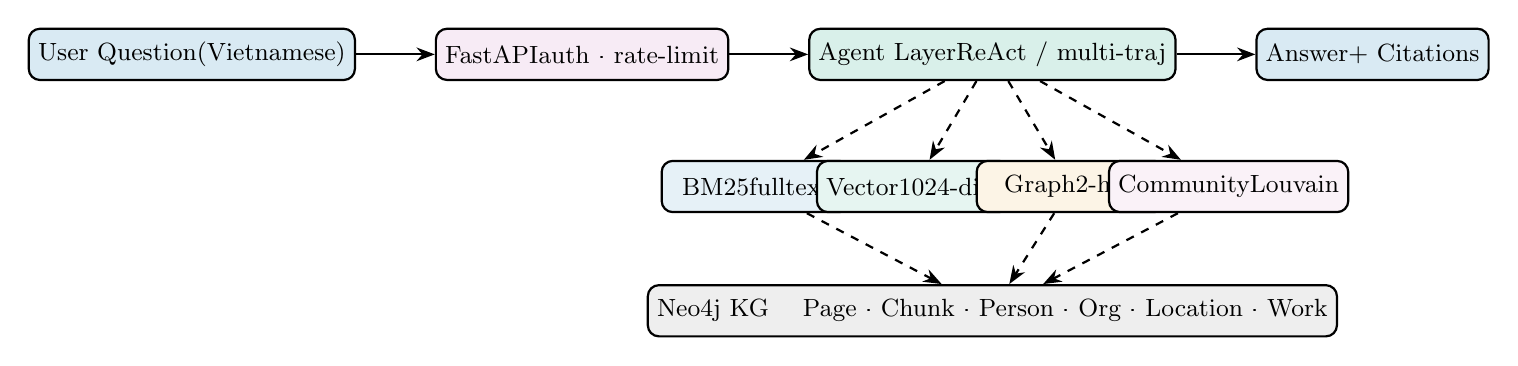
\begin{tikzpicture}[
  box/.style={draw, rounded corners, minimum width=2.4cm, minimum height=0.65cm, font=\small, thick},
  arr/.style={-{Stealth}, thick}
]
  \node[box, fill=positive!15] (query) {User Question\\(Vietnamese)};
  \node[box, fill=cbPurple!15, right=1.0cm of query] (api) {FastAPI\\auth · rate-limit};
  \node[box, fill=emphasis!15, right=1.0cm of api] (agent) {Agent Layer\\ReAct / multi-traj};
  \node[box, fill=positive!15, right=1.0cm of agent] (ans) {Answer\\+ Citations};

  \draw[arr] (query) -- (api);
  \draw[arr] (api) -- (agent);
  \draw[arr] (agent) -- (ans);

  \node[box, fill=positive!10, below=1.0cm of agent, xshift=-3.0cm] (bm25) {BM25\\fulltext};
  \node[box, fill=emphasis!10, below=1.0cm of agent, xshift=-1.0cm] (vec) {Vector\\1024-dim};
  \node[box, fill=negative!10, below=1.0cm of agent, xshift=1.0cm] (graph) {Graph\\2-hop};
  \node[box, fill=cbPurple!10, below=1.0cm of agent, xshift=3.0cm] (comm) {Community\\Louvain};

  \draw[arr, dashed] (agent) -- (bm25);
  \draw[arr, dashed] (agent) -- (vec);
  \draw[arr, dashed] (agent) -- (graph);
  \draw[arr, dashed] (agent) -- (comm);

  \node[box, fill=neutral!15, below=0.9cm of vec, xshift=1.0cm, minimum width=6.5cm] (neo4j)
    {Neo4j KG \quad Page · Chunk · Person · Org · Location · Work};

  \draw[arr, dashed] (bm25) -- (neo4j);
  \draw[arr, dashed] (graph) -- (neo4j);
  \draw[arr, dashed] (comm) -- (neo4j);
\end{tikzpicture}
}
\end{center}
\end{frame}

% SLIDE 7: Requirements
\begin{frame}[shrink=8]{5. Requirements (SRS Summary)}
\textbf{Functional Requirements (Must Have)}
\vspace{2pt}
\begin{center}
\footnotesize
\begin{tabular}{l>{\raggedright\arraybackslash}p{4.5cm}l}
\toprule
\textbf{ID} & \textbf{Requirement} & \textbf{Verifiable By} \\
\midrule
FR-01 & Ingest Vietnamese Wikipedia articles & Unit test \\
FR-02 & Answer single-hop factual questions & EM/F1 on ViQuAD2 \\
FR-03 & Answer multi-hop questions + citations & Hit Rate on ViWiki-MHR \\
FR-04 & Bulk ingest from HuggingFace & Load test 10K articles \\
FR-05 & Generate MHQA evaluation dataset & QC pipeline pass rate \\
\bottomrule
\end{tabular}
\end{center}
\vspace{1pt}
\textbf{Non-Functional Requirements}
\vspace{2pt}
\begin{center}
\footnotesize
\begin{tabular}{llll}
\toprule
\textbf{ID} & \textbf{Metric} & \textbf{Target} & \textbf{Achieved} \\
\midrule
NFR-01 & P50 latency & $<$3s / $<$8s & 51ms retrieval \pos{\checkmark} \\
NFR-02 & Context Hit Rate & $>$70\% & 64.67\% \con{$\sim$} \\
NFR-03 & Test coverage & $\geq$75\% & 85\% \pos{\checkmark} \\
\bottomrule
\end{tabular}
\end{center}
\end{frame}

% SLIDE 8: AI Problem Framing
\begin{frame}[shrink=8]{6. AI: Problem Framing}
\begin{center}
\footnotesize
\begin{tabular}{l>{\raggedright\arraybackslash}p{5.5cm}}
\toprule
\textbf{Layer} & \textbf{Content} \\
\midrule
Business Problem & Complex Vietnamese questions need synthesis across multiple Wikipedia articles \\[1pt]
AI Task & Multi-hop KGQA: Graph-augmented RAG with typed knowledge graph \\[1pt]
Formal Definition & $Q \rightarrow$ retrieve $\{P_1 \ldots P_n\}$ from KG $G$ $\rightarrow$ generate $A$ + citations \\
\bottomrule
\end{tabular}
\end{center}
\vspace{0.1em}
\textbf{Question Taxonomy}
\vspace{1pt}
\begin{center}
\footnotesize
\begin{tabular}{lll}
\toprule
\textbf{Type} & \textbf{Hops} & \textbf{Example} \\
\midrule
Simple (lookup) & 1-hop & ``Born in which year?'' \\
Bridge & 2-hop & ``Where did the founder of [X] study?'' \\
Comparison & 2+ hop & ``Who is older: A or B?'' \\
Fan-out & 3+ hop & ``List all works by [X]'' \\
\bottomrule
\end{tabular}
\end{center}
\vspace{0.4em}
\small \pos{\textbf{Feasibility:}} 15 weeks, team of 4 --- core pipeline already operational \checkmark
\end{frame}

% SLIDE 9: Dataset
\begin{frame}[shrink=5]{7. Dataset}
\begin{center}
\begin{tabular}{llll}
\toprule
\textbf{Dataset} & \textbf{Size} & \textbf{Source} & \textbf{Purpose} \\
\midrule
Vietnamese Wikipedia & $\sim$590K articles & \texttt{wikimedia/wikipedia} & KG construction \\
ViWiki-MHR & $\sim$200 pairs & KG walk + manual & Multi-hop eval \\
UIT-ViQuAD 2.0 & 36,457 pairs & UIT-NLP (VLSP 2021) & Benchmark \\
\bottomrule
\end{tabular}
\end{center}
\vspace{0.4em}
\begin{exampleblock}{Data Quality Pipeline}
\begin{itemize}
  \item \textbf{Stub filtering:} $\geq$200 chars (1.29M $\rightarrow$ $\sim$590K articles)
  \item \textbf{Quality filtering:} redirect, disambiguous, single character articles, dates, lists of articles (index)
  \item \textbf{NFC Unicode normalization} for Vietnamese diacritics
  \item \textbf{5-layer QC:} well-formedness $\rightarrow$ grounding $\rightarrow$ dedup $\rightarrow$ answerability $\rightarrow$ schema
\end{itemize}
\end{exampleblock}
\end{frame}

% SLIDE 10: Related Works Paper 1
\begin{frame}{8. Related Works --- Paper 1}
\begin{block}{Microsoft GraphRAG --- Edge et al., 2024 (arXiv:2404.16130)}
Hierarchical community detection (Leiden) $\rightarrow$ pre-generate community summaries $\rightarrow$ map-reduce at query time. \textbf{Original result:} 70--80\% win rate vs.\ naive RAG on broad queries.
\end{block}
\vspace{0.6em}
\textbf{Applied in this project:}
\begin{itemize}
  \item Louvain community detection $\rightarrow$ assign chunks to communities
  \item Community summaries $\rightarrow$ 4th WRRF signal (weight = 0.15)
  \item Improves recall for broad thematic queries about Vietnamese history/geography
\end{itemize}
\end{frame}

% SLIDE 11: Related Works Paper 2
\begin{frame}{8. Related Works --- Paper 2}
\begin{block}{Inference-Scaled GraphRAG --- Thompson et al., 2025 (arXiv:2506.19967)}
Sample $N$ graph traversal trajectories with temperature scaling $\rightarrow$ aggregate via majority voting.
\textbf{Original result:} Substantial gains over traditional GraphRAG on GRBench; 31.44\% vs.\ 15.26\% on hard multi-hop questions.
\end{block}
\vspace{0.6em}
\textbf{Applied in this project:}
\begin{itemize}
  \item \texttt{AGENT\_N\_TRAJECTORIES} config --- $N$ agents run in parallel with temperature scaling
  \item Majority voting $\rightarrow$ consensus answer
  \item Particularly effective for comparison and fan-out question types
\end{itemize}
\end{frame}

% SLIDE 12: Related Works Paper 3
\begin{frame}[shrink=5]{8. Related Works --- Paper 3}
\begin{block}{UIT-ViQuAD 2.0 --- Nguyen et al., 2020 (arXiv:2009.14725)}
36,457 QA pairs from Vietnamese Wikipedia. Answerable + unanswerable.\\[4pt]
\textbf{Dataset curation:} 5,000 paragraphs from 174 Wikipedia articles; questions manually created per paragraph.\\[4pt]
\textbf{SotA baseline (VLSP 2021):} 77.24\% F1 / 67.43\% EM on private test set.
\end{block}
\vspace{0.4em}
\textbf{Applied in this project:}
\begin{itemize}
  \item Primary benchmark for retrieval quality evaluation
  \item \texttt{src/viquad\_adapter.py} adapts HuggingFace $\rightarrow$ eval pipeline
\end{itemize}
\vspace{0.3em}
\begin{alertblock}{Research Gap}
Single-hop only, no KG walk $\Rightarrow$ need a multi-hop dataset $\Rightarrow$ \textbf{Our ViWikiHop dataset}
\end{alertblock}
\end{frame}

% SLIDE 13: AI Pipeline
\begin{frame}{9. AI Pipeline}
\begin{columns}[T]
\column{0.50\textwidth}
\textbf{Ingestion}
\vspace{6pt}

{\small Wikipedia $\rightarrow$ normalize $\rightarrow$ chunk(500/50) $\rightarrow$ NER $\rightarrow$ embed $\rightarrow$ Neo4j}

\vspace{0.8em}
\textbf{Retrieval (WRRF Fusion)}\\[4pt]
{\small
BM25 ($w$=0.4), Vector ($w$=0.4), Graph ($w$=0.2), Community ($w$=0.15)\\[3pt]
$\rightarrow$ WRRF($k$=60) $\rightarrow$ rerank $\rightarrow$ top-$K$
}

\column{0.45\textwidth}
\textbf{Answer Generation}\\[4pt]
{\small
$Q$ + complexity detection\\[3pt]
\quad $\rightarrow$ \textit{Simple:} ReAct ($\leq$6 iter, 6 tools)\\[3pt]
\quad $\rightarrow$ \textit{Complex:}\\
\quad\quad decompose sub-questions\\
\quad\quad $N$ trajectories (parallel)\\
\quad\quad majority vote\\
\quad\quad $\rightarrow$ $A$ + citations
}
\end{columns}
\end{frame}

% SLIDE 9-vis: AI Pipeline — End-to-End Diagram
\begin{frame}{9. AI Pipeline --- End-to-End Overview}
\centering\vspace{6pt}
\begin{tikzpicture}[scale=0.58, transform shape,
  box/.style={draw=fptNavy, fill=fptNavy!8, rounded corners=5pt,
              font=\normalsize, text width=2.4cm, align=center,
              inner sep=5pt, minimum height=0.85cm},
  db/.style={draw=emphasis!80, fill=emphasis!10, rounded corners=5pt,
             font=\normalsize\bfseries, text width=2.4cm, align=center,
             inner sep=5pt, minimum height=0.85cm},
  src/.style={draw=positive!70, fill=positive!8, rounded corners=4pt,
              font=\normalsize, text width=2.4cm, align=center,
              inner sep=4pt, minimum height=0.8cm},
  out/.style={draw=fptOrange!90, fill=fptOrange!12, rounded corners=5pt,
              font=\normalsize\bfseries, text width=2.4cm, align=center,
              inner sep=5pt, minimum height=0.85cm},
  hdr/.style={font=\large\bfseries, fptOrange!80!black},
  arr/.style={-Stealth, fptNavy, line width=1.5pt},
  darr/.style={-Stealth, fptNavy!40, dashed, line width=1.0pt}
]

% ── Phase labels ─────────────────────────────────────────────────────────
\node[hdr] at (5.5,  5.0) {Ingestion};
\node[hdr] at (12.5, 5.0) {Retrieval};
\node[hdr] at (19.0, 5.0) {Generation};

% ── Ingestion ────────────────────────────────────────────────────────────
\node[box, fill=cbPurple!12] (wiki)  at (0,   3.5) {Wikipedia};
\node[box]  (norm)  at (3.5,  3.5) {Normalize};
\node[box]  (chunk) at (7.0,  3.5) {Chunk};
\node[box]  (ner)   at (10.5, 3.5) {NER};
\node[box]  (embed) at (14.0, 3.5) {Embed};
\node[db]   (neo4j) at (17.5, 3.5) {Neo4j KG};

\draw[arr] (wiki) -- (norm);
\draw[arr] (norm) -- (chunk);
\draw[arr] (chunk) -- (ner);
\draw[arr] (ner) -- (embed);
\draw[arr] (embed) -- (neo4j);

% ── Retrieval + Generation ────────────────────────────────────────────────
\node[box, fill=cbPurple!12] (q)     at (0,    0) {Question};
\node[src] (bm25)   at (3.5,  1.4) {BM25};
\node[src] (vec)    at (3.5,  0)   {Vector};
\node[src] (graph)  at (3.5, -1.4) {Graph};
\node[box] (wrrf)   at (7.5,  0)   {WRRF};
\node[box] (rerank) at (11.5, 0)   {Rerank};
\node[box] (agent)  at (15.5, 0)   {ReAct Agent};
\node[out] (ans)    at (20.0, 0)   {Answer + Citations};

\draw[arr] (q.east) -- ++(1.2,0) |- (bm25.west);
\draw[arr] (q.east) -- ++(1.2,0) |- (vec.west);
\draw[arr] (q.east) -- ++(1.2,0) |- (graph.west);
\draw[arr] (bm25.east)  -- (wrrf.north west|-bm25.east);
\draw[arr] (vec.east)   -- (wrrf.west);
\draw[arr] (graph.east) -- (wrrf.south west|-graph.east);
\draw[arr] (wrrf) -- (rerank);
\draw[arr] (rerank) -- (agent);
\draw[arr] (agent) -- (ans);

% ── KG feeds retrieval ───────────────────────────────────────────────────
\draw[darr] (neo4j.south) -- ++(0,-0.5) -| (bm25.north);
\draw[darr] (neo4j.south) -- ++(0,-0.5) -| (vec.north);
\draw[darr] (neo4j.south) -- ++(0,-0.5) -| (graph.north);

\end{tikzpicture}
\end{frame}

% SLIDE 9a: Stage 1 — Data Ingestion
\begin{frame}[shrink=5]{9a. AI Pipeline --- Stage 1: Data Ingestion}
\vspace{6pt}
\centering
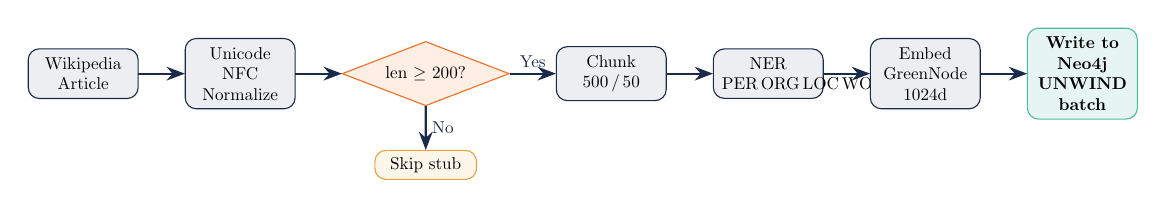
\begin{tikzpicture}[scale=0.62, transform shape,
  node distance=0.45cm and 0.95cm,
  box/.style={draw=fptNavy, fill=fptNavy!8, rounded corners=4pt,
              font=\normalsize, text width=1.9cm, align=center,
              inner sep=5pt, minimum height=0.75cm},
  dec/.style={draw=fptOrange, fill=fptOrange!12, diamond, aspect=2.6,
              font=\normalsize, align=center, inner sep=4pt},
  skip/.style={draw=negative!80, fill=negative!8, rounded corners=4pt,
               font=\normalsize, text width=1.8cm, align=center, inner sep=4pt},
  db/.style={draw=emphasis!70, fill=emphasis!10, rounded corners=4pt,
             font=\normalsize\bfseries, text width=1.9cm, align=center, inner sep=5pt},
  arr/.style={-Stealth, fptNavy, thick}
]
\node[box] (wiki)                    {Wikipedia Article};
\node[box, right=of wiki]  (norm)    {Unicode NFC Normalize};
\node[dec, right=of norm]  (len)     {len $\geq$ 200?};
\node[skip, below=0.9cm of len] (skip) {Skip stub};
\node[box, right=of len]   (chunk)   {Chunk\\500\,/\,50};
\node[box, right=of chunk] (ner)     {NER\\PER\,ORG\,LOC\,WORK};
\node[box, right=of ner]   (embed)   {Embed\\GreenNode\\1024d};
\node[db,  right=of embed] (neo4j)   {Write to Neo4j\\UNWIND batch};
\draw[arr] (wiki)  -- (norm);
\draw[arr] (norm)  -- (len);
\draw[arr] (len)   -- node[above, font=\normalsize]{Yes} (chunk);
\draw[arr] (len)   -- node[right, font=\normalsize]{No}  (skip);
\draw[arr] (chunk) -- (ner);
\draw[arr] (ner)   -- (embed);
\draw[arr] (embed) -- (neo4j);
\end{tikzpicture}

\vspace{8pt}
{\small
\begin{tabular}{@{}lll@{}}
\toprule
\textbf{Stub filter} & \textbf{NER backend} & \textbf{Embedding} \\
\midrule
1.29M $\to$ $\sim$590K articles & \texttt{wikilink} (Typed F1 = 46.9\%) & GreenNode 1024-dim \\
\bottomrule
\end{tabular}}
\end{frame}

% SLIDE 9b: Stage 2 — WRRF Retrieval
\begin{frame}[shrink=5]{9b. AI Pipeline --- Stage 2: WRRF Retrieval}
\begin{columns}[c]
\column{0.52\textwidth}
\centering
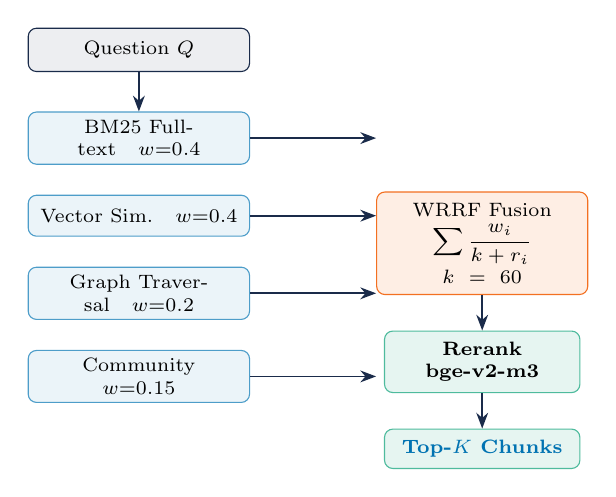
\begin{tikzpicture}[
  node distance=0.38cm and 1.6cm,
  box/.style={draw=fptNavy, fill=fptNavy!8, rounded corners=3pt,
              font=\scriptsize, text width=2.6cm, align=center,
              inner sep=3pt, minimum height=0.55cm},
  src/.style={draw=positive!70, fill=positive!8, rounded corners=3pt,
              font=\scriptsize, text width=2.6cm, align=center,
              inner sep=3pt, minimum height=0.52cm},
  fuse/.style={draw=fptOrange, fill=fptOrange!12, rounded corners=3pt,
               font=\scriptsize, text width=2.4cm, align=center, inner sep=4pt},
  res/.style={draw=emphasis!70, fill=emphasis!10, rounded corners=3pt,
              font=\scriptsize\bfseries, text width=2.2cm, align=center, inner sep=4pt},
  arr/.style={-Stealth, fptNavy, semithick}
]
\node[box]  (q)     {Question $Q$};
\node[src, below=0.5cm of q]  (bm25)  {BM25 Fulltext\quad $w{=}0.4$};
\node[src, below=of bm25]     (vec)   {Vector Sim.\quad $w{=}0.4$};
\node[src, below=of vec]      (graph) {Graph Traversal\quad $w{=}0.2$};
\node[src, below=of graph]    (comm)  {Community\quad $w{=}0.15$};
\node[fuse, right=of vec, yshift=-0.35cm] (wrrf) {WRRF Fusion\\[2pt]$\displaystyle\sum\frac{w_i}{k+r_i}$\\[1pt]$k=60$};
\node[res, below=0.45cm of wrrf] (rnk) {Rerank\\bge-v2-m3};
\node[res, below=0.45cm of rnk]  (topk) {\pos{Top-$K$ Chunks}};
\draw[arr] (q) -- (bm25);
\draw[arr] (bm25.east)  -- (wrrf.west|-bm25.east);
\draw[arr] (vec.east)   -- (wrrf.west|-vec.east);
\draw[arr] (graph.east) -- (wrrf.west|-graph.east);
\draw[arr] (comm.east)  -- (wrrf.west|-comm.east);
\draw[arr] (wrrf) -- (rnk);
\draw[arr] (rnk)  -- (topk);
\end{tikzpicture}

\column{0.45\textwidth}
\textbf{Fusion Formula}\\[4pt]
{\small$\text{score}(d) = \displaystyle\sum_{i} \frac{w_i}{k + \text{rank}_i(d)}$}\\[8pt]
\begin{tabular}{ll}
\toprule
\textbf{Signal} & \textbf{Weight} \\
\midrule
BM25 Fulltext  & 0.40 \\
Vector (cosine)& 0.40 \\
Graph 2-hop    & 0.20 \\
Community      & 0.15 \\
\bottomrule
\end{tabular}\\[8pt]
{\small $k=60$ smooths rank-1 dominance.\\
Final reranker: BAAI/bge-reranker-v2-m3 (cross-encoder).}
\end{columns}
\end{frame}

% SLIDE 9c: Stage 3 — Answer Generation
\begin{frame}[shrink=5]{9c. AI Pipeline --- Stage 3: Answer Generation}
\centering\vspace{4pt}
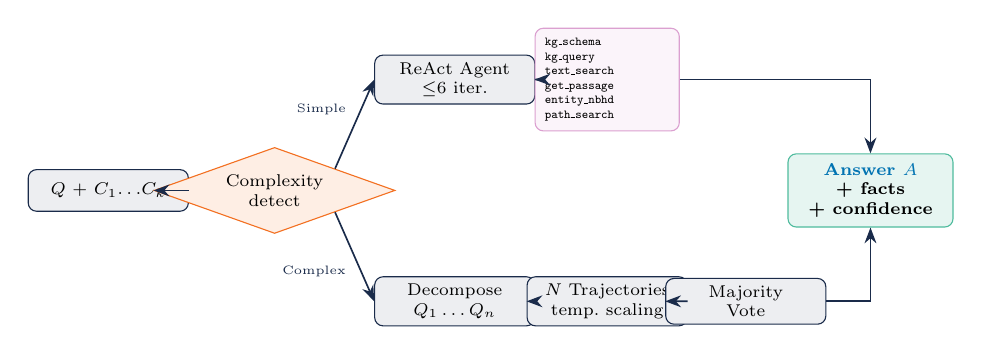
\begin{tikzpicture}[scale=0.88, transform shape,
  box/.style={draw=fptNavy, fill=fptNavy!8, rounded corners=3pt,
              font=\scriptsize, text width=2.1cm, align=center,
              inner sep=3pt, minimum height=0.6cm},
  dec/.style={draw=fptOrange, fill=fptOrange!12, diamond, aspect=2.8,
              font=\scriptsize, align=center, inner sep=3pt},
  tools/.style={draw=cbPurple!70, fill=cbPurple!8, rounded corners=3pt,
                font=\tiny, text width=1.8cm, align=left, inner sep=4pt},
  res/.style={draw=emphasis!70, fill=emphasis!10, rounded corners=3pt,
              font=\scriptsize\bfseries, text width=2.1cm, align=center, inner sep=4pt},
  arr/.style={-Stealth, fptNavy, semithick}
]
\node[box]   (in)     at (0,    0)    {$Q$ + $C_1\!\ldots\!C_k$};
\node[dec]   (cd)     at (2.4,  0)    {Complexity\\detect};
\node[box]   (react)  at (5,    1.6)  {ReAct Agent\\ $\leq$6 iter.};
\node[tools] (tools)  at (7.2,  1.6)  {%
  \texttt{kg\_schema}\\
  \texttt{kg\_query}\\
  \texttt{text\_search}\\
  \texttt{get\_passage}\\
  \texttt{entity\_nbhd}\\
  \texttt{path\_search}};
\node[box]   (decomp) at (5,   -1.6)  {Decompose\\$Q_1\ldots Q_n$};
\node[box]   (traj)   at (7.2, -1.6)  {$N$ Trajectories\\temp.\ scaling};
\node[box]   (vote)   at (9.2, -1.6)  {Majority\\Vote};
\node[res]   (ans)    at (11,   0)    {\pos{Answer $A$}\\+ facts\\+ confidence};
\draw[arr] (in) -- (cd);
\draw[arr] (cd.north east) -- node[above left, font=\tiny]{Simple}  (react.west);
\draw[arr] (cd.south east) -- node[below left, font=\tiny]{Complex} (decomp.west);
\draw[arr] (react)  -- (tools);
\draw[arr] (decomp) -- (traj);
\draw[arr] (traj)   -- (vote);
\draw[arr] (tools.east) -| (ans.north);
\draw[arr] (vote.east)  -| (ans.south);
\end{tikzpicture}
\end{frame}

% SLIDE 10: Evaluation Metrics
\begin{frame}[shrink=15]{10. Evaluation Metrics}
\begin{columns}[T]
\column{0.50\textwidth}
\textbf{Exact Match (EM)}\\[3pt]
{\small Binary: 1 if predicted answer matches any gold answer exactly (after normalization), 0 otherwise.}\\[2pt]
{\small $\displaystyle\text{EM} = \frac{1}{N}\sum_{i=1}^{N}\mathbf{1}[\hat{a}_i = a_i]$}\\[2pt]
{\small Normalization: lowercase, strip punctuation \& articles.}

\vspace{0.6em}
\textbf{Token F1}\\[3pt]
{\small Soft overlap between predicted and gold answer token bags.}\\[2pt]
{\small $\displaystyle F_1 = \frac{2 \cdot P \cdot R}{P + R}$, \quad $P = \frac{|\hat{T} \cap T|}{|\hat{T}|}$, \quad $R = \frac{|\hat{T} \cap T|}{|T|}$}

\column{0.46\textwidth}
\textbf{Benchmark: UIT-ViQuAD 2.0}\\[4pt]
\begin{itemize}
  \item 36{,}457 QA pairs from Vietnamese Wikipedia
  \item Answerable + unanswerable questions
  \item Standard MRC evaluation protocol (SQuAD-style)
\end{itemize}
\vspace{0.4em}
\begin{block}{SotA Reference (VLSP 2021)}
\begin{center}
\footnotesize
\begin{tabular}{lll}
\toprule
\textbf{Model} & \textbf{EM} & \textbf{F1} \\
\midrule
XLM-R (fine-tuned) & 67.43\% & 77.24\% \\
\bottomrule
\end{tabular}
\end{center}
\end{block}
\vspace{0.3em}
{\small Our system targets comparable F1 after full corpus ingestion ($\sim$590K articles).}
\end{columns}
\end{frame}

% SLIDE 14: Baselines & Results (hidden)
\iffalse
\begin{frame}{10. Baselines \& Results}
\begin{center}
\begin{tabular}{llll}
\toprule
\textbf{Method} & \textbf{MRR} & \textbf{Hit Rate@5} & \textbf{Latency} \\
\midrule
BM25 only & $\sim$0.35 & $\sim$55\% & 0.8s \\
Dense only & $\sim$0.40 & $\sim$60\% & 1.2s \\
Naive RAG & $\sim$0.42 & $\sim$62\% & 2.5s \\
BM25 + Vector & $\sim$0.48 & $\sim$66\% & 1.5s \\
\midrule
\pos{\textbf{Ours (WRRF+Rerank)}} & \pos{\textbf{0.4497}} & \pos{\textbf{64.67\%}} & \pos{\textbf{51ms}} \\
\bottomrule
\end{tabular}
\end{center}
\vspace{0.4em}
\begin{columns}[T]
\column{0.48\textwidth}
\begin{exampleblock}{Strong Results}
+$\sim$20\% MRR vs.\ best baseline\\
Retrieval latency 51ms (ViQuAD2, 2,652 queries)\\
Test coverage: 85\% \pos{\checkmark}
\end{exampleblock}
\column{0.48\textwidth}
\begin{alertblock}{Gap to Close}
Hit Rate 64.67\% $<$ 70\% target\\
\con{Root cause:} full ingestion needed for sufficient entity coverage in KG
\end{alertblock}
\end{columns}
\end{frame}
\fi

% SLIDE 15: Team Assignment
\begin{frame}{11. Team Assignment}
\begin{center}
\small
\begin{tabular}{ll>{\raggedright\arraybackslash}p{6.2cm}}
\toprule
\textbf{Member} & \textbf{ID} & \textbf{Responsibility} \\
\midrule
Huynh Quoc Trung & QE180038 & KG Construction · NER (6 backends) · Entity Resolution \\
Nhu Quang Anh & QE180005 & WRRF Retrieval · Reranker · Evaluation Pipeline \\
Pham Ngo Dinh Khoi & QE180110 & ReAct Agent · Local LLM · MHQA Dataset Gen \\
Truong Dinh Thien & QE180018 & FastAPI · Job Management · Gradio Demo · Deploy \\
\bottomrule
\end{tabular}
\end{center}
\vspace{0.6em}
\begin{block}{Dependency Chain}
\centering
NER (Trung) $\rightarrow$ Entity quality $\rightarrow$ Graph signal (Anh) $\rightarrow$ Agent tools (Khoi) $\rightarrow$ FastAPI (Thien)
\end{block}
\end{frame}

% SLIDE 16: System Scale & Timeline
\begin{frame}{12. System Scale \& Timeline}
\begin{block}{Use Case Points}
\textbf{UCP = 96.5} \quad (UUCP = 134 · TCF = 0.9 · ECF = 0.8) \quad $\rightarrow$ Feasible in 15 weeks \pos{\checkmark}
\end{block}
\vspace{0.5em}
\begin{center}
\begin{tabular}{ll>{\raggedright\arraybackslash}p{5.5cm}}
\toprule
\textbf{Week} & \textbf{Milestone} & \textbf{Status} \\
\midrule
1--4 & Core pipeline + SRS + Architecture & \pos{Done \checkmark} \\
5--7 & Full ingestion + Ablation + MHQA & \con{In progress $\sim$} \\
8--10 & QLoRA Text2Cypher + DPO alignment & Pending \\
11--13 & WRRF tuning + final evaluation & Pending \\
14--15 & Final report + demo + defense & Pending \\
\bottomrule
\end{tabular}
\end{center}
\end{frame}

% SLIDE 17: Thank You
\begin{frame}[plain]
\begin{center}
\vspace{2cm}
{\Huge \textbf{Thank You}}\\[1em]
{\Large Questions \& Discussion}\\[2em]
{\normalsize Vietnamese GraphRAG --- Multi-hop QA over Vietnamese Wikipedia}\\[0.5em]
{\small \textcolor{neutral}{Local-first $\cdot$ Multi-hop $\cdot$ Citation-grounded $\cdot$ Fully local GPU}}
\end{center}
\end{frame}

% BACKUP SLIDES
\backupbegin
\appendix

\begin{frame}{Appendix: Graph Schema}
\begin{columns}[T]
\column{0.50\textwidth}
\textbf{Node \& Edge Types}\\[6pt]
{\small\ttfamily
(:Page) -[:HAS\_CHUNK]$\rightarrow$ (:Chunk)\\[2pt]
(:Chunk)-[:MENTIONS\_PERSON]$\rightarrow$(:Person)\\
(:Chunk)-[:MENTIONS\_ORG]$\rightarrow$(:Organization)\\
(:Chunk)-[:MENTIONS\_LOC]$\rightarrow$(:Location)\\
(:Chunk)-[:MENTIONS\_WORK]$\rightarrow$(:Work)\\[2pt]
(:Page) -[:LINKS\_TO]$\rightarrow$ (:Page)
}

\column{0.45\textwidth}
\textbf{Indexes}
\begin{itemize}
  \item Fulltext index on \texttt{chunk.text}
  \item Vector index on \texttt{chunk.embedding} (1024-dim)
  \item B-tree index on \texttt{entity.name}
\end{itemize}
\vspace{0.4em}
\textbf{Current scale:}\\
998 pages · 19K chunks · 3.3K entities
\end{columns}
\end{frame}

\begin{frame}{Appendix: WRRF Formula}
\begin{block}{Weighted Reciprocal Rank Fusion}
\[
\text{score}(d) = \sum_i \frac{w_i}{k + \text{rank}_i(d)}
\]
\[
k = 60 \quad w_{\text{BM25}} = 0.4 \quad w_{\text{Vector}} = 0.4 \quad w_{\text{Graph}} = 0.2 \quad w_{\text{Community}} = 0.15
\]
\end{block}
\vspace{0.5em}
\textbf{Cross-encoder reranker:} \texttt{BAAI/bge-reranker-v2-m3}\\
Rescores top-20 candidates $\rightarrow$ returns top-5 to the agent
\end{frame}

\begin{frame}{Appendix: NER Backend Comparison}
\begin{center}
\begin{tabular}{lll}
\toprule
\textbf{Backend} & \textbf{Method} & \textbf{Best Use} \\
\midrule
Simple & Regex + keyword & Fast, no GPU \\
Underthesea & BIO tagging & Offline, general \\
PhoNLP & VnCoreNLP + PhoNLP & Accurate, slow \\
PhoBERT & Transformer pipeline & High accuracy \\
ViDeBERTa & Electra-base NER & Balanced \\
\HL{Wikilink} & Hyperlink extraction & \HL{Bulk ingestion (Typed F1 = 46.9\%)} \\
\bottomrule
\end{tabular}
\end{center}
\vspace{0.4em}
All backends output \texttt{(name, type)} tuples $\rightarrow$ typed graph labels\\
Postprocessing: noise filter $\rightarrow$ org reclassification $\rightarrow$ deduplication
\end{frame}

\backupend

\end{document}
